\documentclass{manuscript}

\usepackage[hidelinks]{hyperref}
\usepackage{textcomp}
\usepackage{amsmath}
\usepackage{pgfplots}
\usepackage{amssymb}
\usepackage{indentfirst}
\usepackage{subcaption}
\usepackage{wrapfig}
\usepackage{enumitem}

\pgfplotsset{compat=1.15}

\title{A Study of The Equipments Market in The E-Sim Game}
\author{Zhang Shiwei}
\date{December 2017}

\begin{document}
    \maketitle

    \section{Introduction}

    \subsection{The E-Sim game}

    The \href{https://www.e-sim.org}{E-Sim} game is a boring browser game where you work everday to make weapons and
    use them to fight for the country you born for no reason. The most important stat of a player is how many damage
    they can make, which in turn depends mostly on their strength and equipments. Since the first game server,
    \href{https://primera.e-sim.org}{\textit{primera}}, has already been runing for more than 6 years, most players have similar
    strength about 3200\verb!+!, which almost don't grow anymore, so equipments is the dominant parameter of a character.

    \subsection{Equipments}

    \begin{wrapfigure}{r}{0.3\textwidth}
        \centering
        \vspace{-1\baselineskip}
        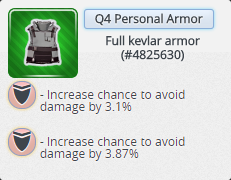
\includegraphics[width=0.28\textwidth]{equipment_example.png}
        \caption{Example of an equipment}\label{fig:equip_exp}
    \end{wrapfigure}

    Each character can equip an equipment on each of his 8 slots. Equipments have 6 qualities: Q1 - Q6. Equipments last
    forever until being merged or split by it's owner. A player can get equipments by battle drops, buying from others
    and special events. Each equipment have 2 parameters, which are generated randomly accroding to it's type and quality.

    Players can merge and split their equipments to make new ones. Merging takes 3 equipments of the same quality and makes
    an new equipments of higher quality. The 3 materials are destroyed from the game. The parameters of the new equipment
    is random, but it's slot is same as one of the materials. For example, you can merge 2 Q2 Helmets with a Q2 Vision,
    and you will get a Q3 Helmet or a Q3 Vision, whose parameters, however, are totally random and independent of the
    materials. The game charges a fee for merging equipments.

    Splitting is basically the reverse of merging. Players can split an equipment of at lease Q2 into 2 equipments of
    lower qualities. One of the new equipments is guaranteed to be on the same slot of the one split. Splitting charges
    no fee.

    \subsection{The Auction}

    The auction in game is where players trade thier assets like companies, drugs and equipments. The currency used in
    the auction is glod, refered to as ``g''. The auction uses the Vickrey mechanism, aka. \textit{sealed-bid second-price
    auction}. Players can put their equipments on the auction with an intial price. Others can bid for any price higher
    than the current. The current price is ether the initial price or the second top offer. The actual price of the top
    offer, however, is hidden. When a sell ends, the top bidder will get the asset for the current price, and the remaining
    part will be returned to him. A typical auction last for 24 hours. The seller can cancel a sell as long as no one
    gave an offer yet.

    The game charges 2\% of the initial price when creating an aution and 1\% of the final price when the auction ends.

    \subsection{Some Definitions}

    \textbf{Defective}: There are three types of parameters of equipments, those increasing damage by absolute values,
    those increasing damage by percentages, and those related to economics. Since the game have been runing for over 6
    years, most players have very high stats, thus increasing damage by percentage is significantly better than increasing
    by absolute value. As a result, no player wear equipments that increasing absolute stats seriously. I call the equipments
    that have at least one parameter of this type \textit{defectives}.

    \textbf{Material}: Still, as a result of the game having been running so long, players have a lot of money but limited
    slots. So no one will wear equipments of low qualities. The only usage of the low quality equipments is being the
    meterials of merging. I call equipments whose average price is below 10g \textit{materials}. Precisely, they are:
    \begin{itemize}[nosep]
        \item Q1 Pants, Shoes, Lucky charms and Personal armors
        \item Q1 and Q2 Offhands
        \item Q1 - Q3 Helmets, Visions and Weapon upgrades
    \end{itemize}

    \section{Equipment Appraisal}

    \subsection{Regression of price $\sim$ quality}

    \begin{figure}[h]
        \centering
        \begin{subfigure}{0.45\textwidth}
            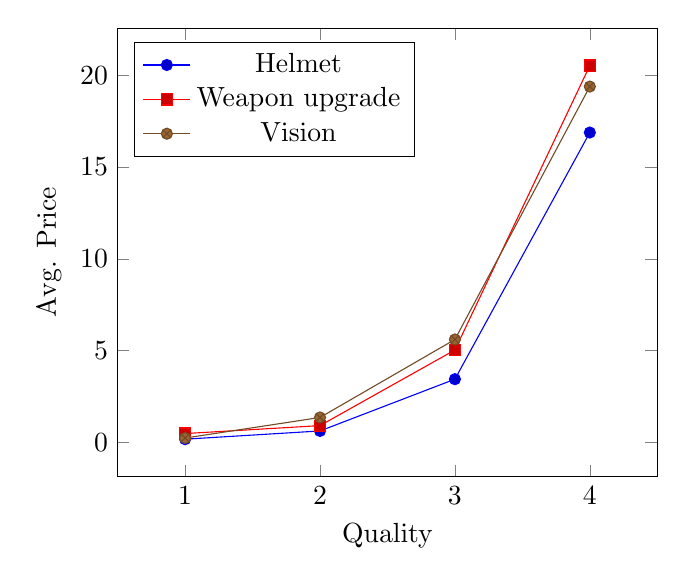
\begin{tikzpicture}
                \begin{axis}[
                    xlabel={Quality},
                    ylabel={Avg. Price},
                    xmin=0.5, xmax=4.5,
                    legend entries={Helmet, Weapon upgrade, Vision},
                    legend pos=north west
                ]
                    \addplot
                    coordinates {
                        (1, 0.1875938402309923)
                        (2, 0.6356372549019648)
                        (3, 3.453225806451614)
                        (4, 16.87775280898877)
                    };
                    \addplot
                    coordinates {
                        (1, 0.49335483870967733)
                        (2, 0.9264179104477622)
                        (3, 5.042137931034481)
                        (4, 20.52022222222223)
                    };
                    \addplot
                    coordinates {
                        (1, 0.2500585937500004)
                        (2, 1.369263157894737)
                        (3, 5.61398734177215)
                        (4, 19.378390804597707)
                    };
                \end{axis}
            \end{tikzpicture}
            \caption{the absolute price}
        \end{subfigure}
        \begin{subfigure}{0.45\textwidth}
            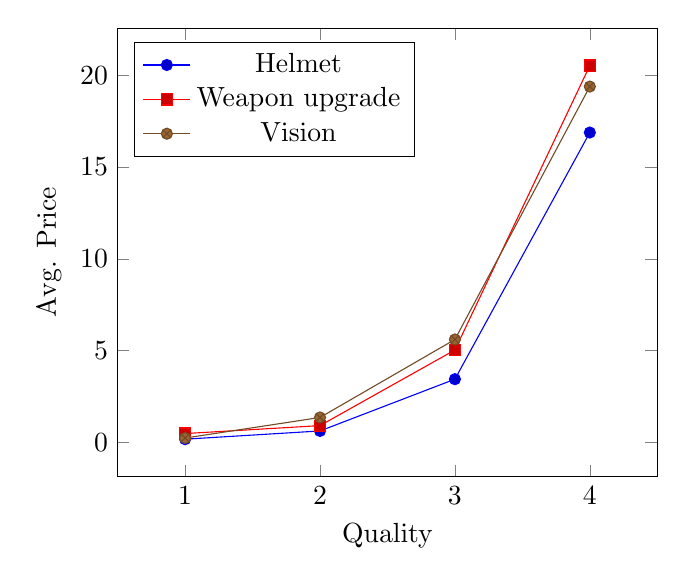
\begin{tikzpicture}
                \begin{axis}[
                    xlabel={Quality},
                    ylabel={Avg. Price},
                    xmin=0.5, xmax=4.5,
                    legend entries={Helmet, Weapon upgrade, Vision},
                    legend pos=north west
                ]
                    \addplot
                    coordinates {
                        (1, 0.1875938402309923)
                        (2, 0.6356372549019648)
                        (3, 3.453225806451614)
                        (4, 16.87775280898877)
                    };
                    \addplot
                    coordinates {
                        (1, 0.49335483870967733)
                        (2, 0.9264179104477622)
                        (3, 5.042137931034481)
                        (4, 20.52022222222223)
                    };
                    \addplot
                    coordinates {
                        (1, 0.2500585937500004)
                        (2, 1.369263157894737)
                        (3, 5.61398734177215)
                        (4, 19.378390804597707)
                    };
                \end{axis}
            \end{tikzpicture}
            \caption{the relative price}
        \end{subfigure}
        \caption{The average price of material equipments}\label{fig:reg1}
    \end{figure}
\end{document}
